\capitulo{3}{Conceptos teóricos}

\section{Machine Learning y Deep Learning}
La base del proyecto se debe al uso del \emph{deep learning}, una rama del \emph{machine learning}.

\subsection{Machine Learning}
El \emph{machine learning}, o en español, aprendizaje automático, busca como principal objetivo desarrollar técnicas o algoritmos que permitan a un computador aprender, a partir de unos datos iniciales.

El proceso es similar al utilizado por animales y humanos para aprender en base a la experiencia, de forma que cuantos más datos se usen para entrenar un algoritmo, mejores resultados se obtengan.

El uso del \emph{machine learning} se debe de emplear en problemas donde nos encontremos con muchos casos diferentes y con multitud de posibilidades y no se encuentre una forma de normalizar de forma matemática todas las posibles opciones.

De forma simple, el esquema \cite{mitchell1997machine} que sigue cualquier método de aprendizaje automático se puede ver en la Figura \ref{esquemaML}.

\begin{figure}[h]
    \centering
    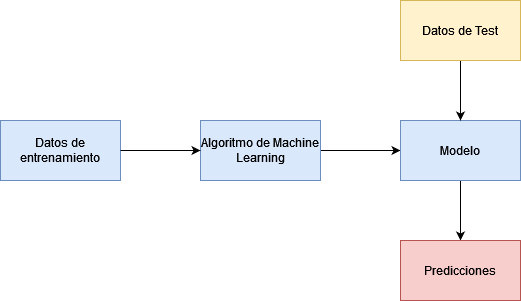
\includegraphics[scale=0.7]{img/Esquema_ML.png}
    \caption{Esquema Algoritmos Machine Learning (Realización Propia).}
    \label{esquemaML}
\end{figure}

\subsection{Deep Learning}
El \emph{deep learning}, en español, aprendizaje profundo, se inspira en el funcionamiento del sistema nervioso humano, donde existen multitud de redes neuronales especializadas en tareas distintas.

Debido a ello, el \emph{deep learning} crea arquitecturas neuronales de forma de que haya zonas encargadas en detectar ciertas características especificas en los datos. Esto ha supuesto grandes mejoras frente a otros tipos de \emph{machine learning} basados en redes artificiales monolíticas.

\section{Visión Artificial}
La visión artificial \cite{eswiki:141758410}, o en inglés, \emph{computer vision}, tiene como objetivo identificar los elementos de las imágenes con el fin de extraer información útil con la que pueda trabajar un ordenador. Busca recrear el proceso que hacen las personas al observar un objeto y saber identificarlo de los demás, pero en este caso, dicho proceso lo hará de forma automática un computador.

\subsection{Segmentación}
La segmentación \cite{palomino2009tecnicas} es una técnica empleada en la visión artificial, la cual consiste en identificar y dividir una imagen en los diferentes objetos que la componen, de modo que, se puedan extraer aquellos con mayor interés.

\section{Redes Neuronales Artificiales}
Las redes neuronales artificiales son un conjunto de neuronas artificiales conectadas entre sí que permiten transmitir señales entre ellas. El principal objetivo de estas redes es resolver problemas como lo hacen los tejidos neuronales biológicos.

En una red neuronal artificial, dos neuronas están conectadas entre sí por un enlace. Dichos enlaces suelen tener un peso asociado, de forma que otras neuronas puedan activarse según los diferentes pesos de las señales que reciben.

La principal ventaja de estas redes es que aprenden solas y no es necesaria su programación paso por paso, ya que la propia red busca minimizar una función de pérdida de la red al completo, consiguiendo que sea capaz de encontrar el mejor camino para cada caso.

\begin{figure}[h]
 \centering
  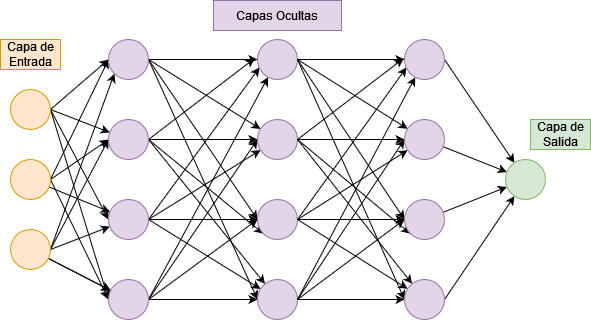
\includegraphics[width=0.8\textwidth]{img/RedNeuronal.png}
 \caption{Ejemplo Red Neuronal Artificial (Realización Propia)}
 \label{f:redneuronal}
\end{figure}

Existen dos tipos de redes neuronales artificiales:
\begin{itemize}
    \item \textbf{Red Neuronal Prealimentada:} son un tipo de red neuronal que no permite bucles, es decir, la información siempre va de izquierda a derecha, como se aprecia en la Figura \ref{f:redneuronal}, de modo que la información siempre va de la capa de entrada a la de salida pasando por las capas ocultas, y nunca pueden volver hacia atrás.
    \item \textbf{Red Neuronal Recurrente:} son un tipo de red que permite bucles, de forma que si se puede volver hacia atrás en las capas. Esto permite a la red tener memoria de los datos recibidos por la neurona anterior.
\end{itemize}

\subsection{Redes Neuronales Convolucionales}
Las redes neuronales convolucionales \cite{castilla2021reconocimiento}, o CNN (del inglés \emph{Convolutional Neural Network}), son el tipo más extendido de redes en computadores para poder darles la capacidad de reconocimiento de los elementos de imágenes y vídeos.

El funcionamiento de las mismas se debe a dos operaciones básicas: convolución y \emph{pooling}.

\subsubsection{Convolución}
Esta operación utiliza una matriz llamada \emph{kernel} que recorre cada uno de los píxeles de la imagen y obtiene un valor calculado (producto escalar) por el píxel que esta procesando junto con todos los que rodean al mismo, y de esta forma se va completando dicha matriz.

Cabe destacar que la nueva matriz obtenida tiene menor tamaño que la imagen original, como se puede ver en la Figura \ref{f:convo}. También, este proceso se puede ir repitiendo varias veces obteniendo una matriz \emph{kernel} de dimensiones menores.

\begin{figure}[h]
 \centering
  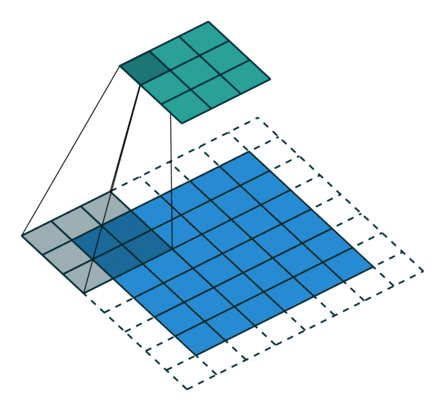
\includegraphics[width=0.6\textwidth]{img/Convo.png}
 \caption{Operación de Convolución \cite{wiki:convo}}
 \label{f:convo}
\end{figure}

\subsubsection{Pooling}
La operación \emph{pooling} se encarga principalmente de obtener dimensiones menores e ir obteniendo las características principales en cada caso.

Esta operación es muy sencilla. En primer lugar, se divide la imagen en una cuadrícula de un tamaño específico cada una. A continuación, por cada cuadrícula se devuelve un valor (generalmente el valor máximo o el valor medio).

La Figura \ref{f:pooling} muestra un ejemplo de la operación \emph{pooling} con una cuadrícula de 2x2 y devolviendo el tamaño máximo de cada celda.

\begin{figure}[h]
 \centering
  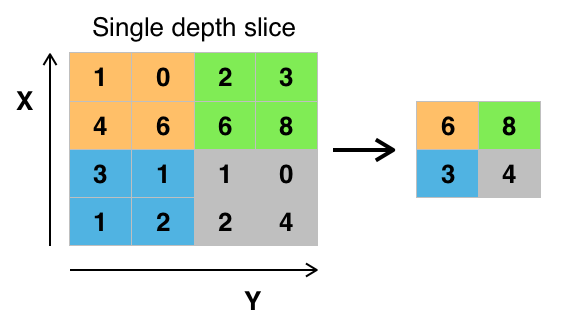
\includegraphics[width=0.6\textwidth]{img/pooling.png}
 \caption{Operación de \emph{Pooling} \cite{wiki:pooling}}
 \label{f:pooling}
\end{figure}

\subsection{R-CNN}
Las CNN son unas redes muy costosas de entrenar en aquellos casos donde las imágenes cuentan con muchas regiones diferentes. Es por ello, que surgen las R-CNN, del inglés \emph{Regions with CNN features}.

La principal diferencia entre las R-CNN y las CNN, es que las primeras tienen la capacidad de detectar varios objetos en una imagen, mientras que el segundo tipo tan solo puede clasificar las imágenes pero sin saber exactamente donde se encuentra el elemento detectado. 

Esto se debe a que en las redes R-CNN existe un algoritmo que divide en pequeñas regiones la imagen e intenta identificar en cada una de las regiones los objetos que sabe detectar. De este modo siempre sabe en que región o regiones se encuentra cada elemento.

\subsection{Faster R-CNN}
Las \emph{Faster R-CNN} suponen una mejora de velocidad en el rendimiento y mejoras en la detección de objetos con respecto a su antecesora R-CNN. Los tiempos que tardan en realizar la predicción estas redes son de alrededor de 0.2 segundos, mientras que las R-CNN tiene un tiempo de entre 40-50 segundos, por lo que se ve claramente la mejora en cuanto a tiempo.

La red \emph{Faster R-CNN} contiene un RPN (\emph{Region Proposal Network}) que permite crear un conjunto de regiones. Esta regiones se crean a través de una capa nueva, denominada ROI (\emph{Region Of Interest}), que permite extraer vectores de regiones y delimitar zona en las imágenes que podrían contener objetos. Todo esto permite obtener mejoras muy considerables en la detección. 

\begin{figure}[h]
 \centering
  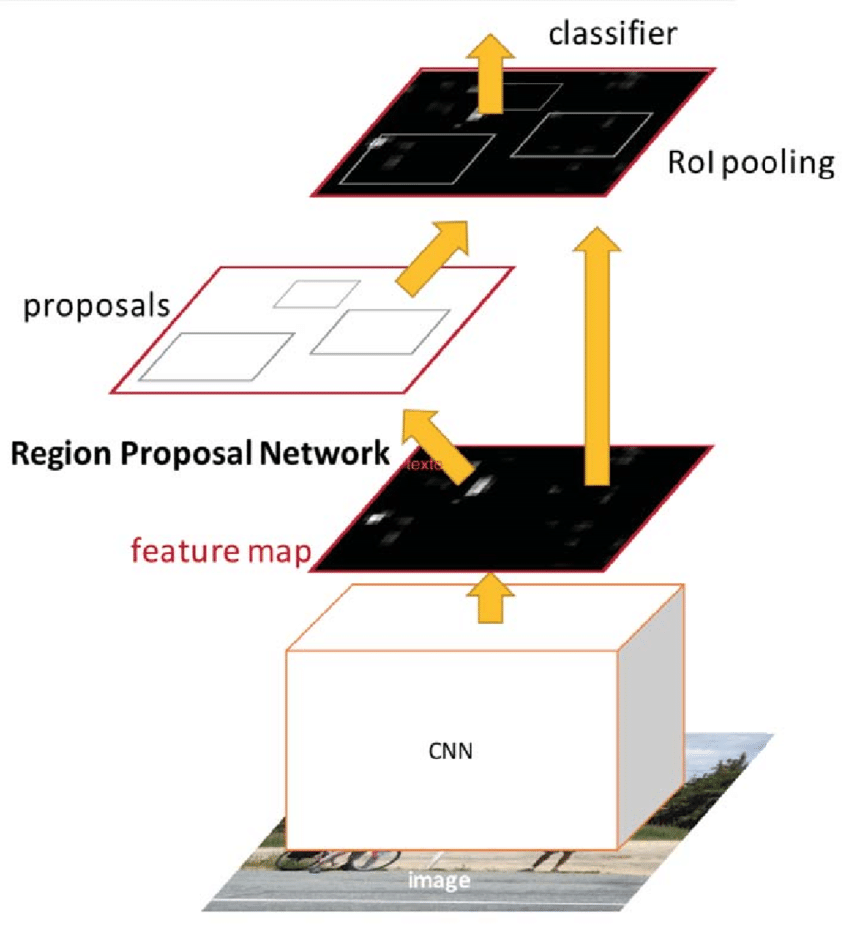
\includegraphics[width=0.6\textwidth]{img/FRCNN.png}
 \caption{Funcionamiento Faster R-CNN \cite{renNIPS15fasterrcnn}}
 \label{f:frcnn}
\end{figure}

\subsection{Mask R-CNN}
\label{mask}
Las redes \emph{Mask R-CNN} son una continuación de las redes \emph{Faster R-CNN}. La principal mejora que trae es que este tipo de redes son capaces de obtener la máscara del objeto detectado, mientras que sus antecesoras tan solo podían identificar los elementos a través de una figura dibujada en la imagen.

Este es el tipo de red neuronal utilizada a lo largo del proyecto, ya que las detecciones por parte del modelo de \emph{Detectron2} funcionan de este modo.

\emph{Detectron2} es una librería de \emph{Python}, desarrollada por \emph{Facebook}, basada en \emph{PyTorch} para la creación de modelos y la segmentación de elementos.

\section{COCO (Common Objects in COntext)}
\label{COCO}
Para poder trabajar con \emph{Detectron2} es necesaria tener la segmentación de las diferentes imágenes en formato COCO. Dicho formato, se basa en tener la segmentación en un JSON con diferentes atributos para poder reconstruir la parte segmentada sin la necesidad de almacenarla de forma original (máscara binaria), y poder trabajar con ella de forma más cómoda.

Existen varios tipos de anotaciones, pero en este proyecto se ha utilizado la formada por los siguientes atributos:
\begin{itemize}
    \item \texttt{file\_name:} contiene el nombre de la imagen a la que referencia dicha segmentación.
    \item \texttt{height:} contiene el valor correspondiente a la altura de la imagen.
    \item \texttt{width:} contiene el valor correspondiente a la anchura de la imagen.
    \item \texttt{annotations:} es un diccionario que contiene los siguientes atributos:
    \begin{itemize}
        \item \texttt{bbox:} contiene los puntos máximos y mínimos en el eje horizontal y vertical, de modo que se pueda generar la caja que contiene en su interior la zona segmentada de dicha imagen.
        \item \texttt{bbox\_mode:} el formato que tiene el atributo anterior, es decir, cada valor se indica a que eje corresponde y cuál es el valor mínimo y cuál el máximo.
        \item \texttt{segmentation:} lista que contiene todos los puntos que dan lugar mediante su unión a la zona segmentada del diente.
        \item \texttt{category\_id:} identificador de la categoría a la que se corresponde dicha segmentación.
    \end{itemize}
\end{itemize}

\section{IoU (Intersection Over Union)}
La técnica IoU se utiliza principalmente para comprobar como de buena ha sido la segmentación producida por un modelo con respecto a la segmentación real. 

En definitiva, mide cuanto están solapadas ambas segmentaciones, tomando valores comprendidos entre el  0 y el 1, siendo este último el mejor valor, indicando que ambas segmentaciones están totalmente solapadas, y 0 que no se solapan, y que por ello la predicción no ha sido muy buena.

A nivel matemático, la formula para obtener el valor de IoU entre dos segmentaciones $A$ y $B$ sería:

$$\textit{IoU(A,B)} = \frac{\left | A \cap B \right |}{\left | A\cup B \right |}$$

